%!TEX root =../../course-notes.tex
% ^ leave for LaTeXTools build functionality

\begin{module}{Module V: Vector Spaces}

\begin{moduleStandards}
  \item \textbf{V1: Vector Spaces.}
        Determine if a set with given operations forms a vector space.
  \item \textbf{V2: Linear Combinations.}
        Determine if a vector can be written as a linear combination of
        a given set of vectors.
  \item \textbf{V3: Spanning Sets.}
        Determine if a set of vectors spans a vector space.
  \item \textbf{V4: Subspaces.}
        Determine if a subset of a vector space is a subset or not.
\end{moduleStandards}

%!TEX root =../../course-notes.tex
% ^ leave for LaTeXTools build functionality

\newcommand{\systemWithOneSolutionA}{
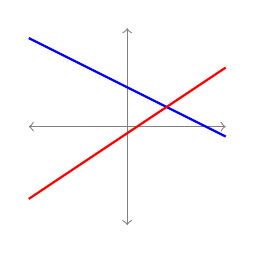
\begin{tikzpicture}[scale=0.25]
\draw[thin,gray,<->] (-5,0) -- (5,0);
\draw[thin,gray,<->] (0,-5) -- (0,5);
\draw[thick,blue] (-5,4.5) -- (5,-0.5);
\draw[thick,red] (-5,-3.67) -- (5,3);
\end{tikzpicture}
}

\newcommand{\systemWithOneSolutionB}{
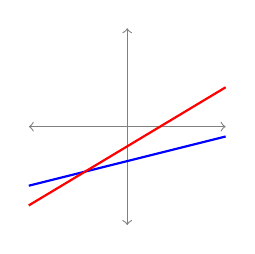
\begin{tikzpicture}[scale=0.25]
\draw[thin,gray,<->] (-5,0) -- (5,0);
\draw[thin,gray,<->] (0,-5) -- (0,5);
\draw[thick,blue] (-5,-3) -- (5,-0.5);
\draw[thick,red] (-5,-4) -- (5,2);
\end{tikzpicture}
}

\newcommand{\systemWithInfinitelyManySolutions}{
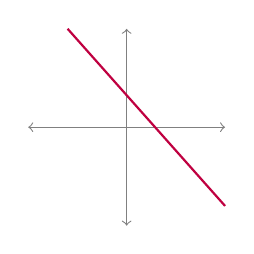
\begin{tikzpicture}[scale=0.25]
\draw[thin,gray,<->] (-5,0) -- (5,0);
\draw[thin,gray,<->] (0,-5) -- (0,5);
\draw[thick,purple] (-3,5) -- (5,-4);
\end{tikzpicture}
}

\newcommand{\systemWithNoSolutions}{
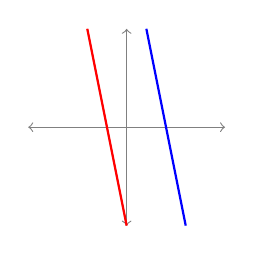
\begin{tikzpicture}[scale=0.25]
\draw[thin,gray,<->] (-5,0) -- (5,0);
\draw[thin,gray,<->] (0,-5) -- (0,5);
\draw[thick,blue] (3,-5) -- (1,5);
\draw[thick,red] (0,-5) -- (-2,5);
\end{tikzpicture}
}

%!TEX root =../../course-notes.tex
% ^ leave for LaTeXTools build functionality

\begin{readinessAssuranceOutcomes}
\item Add Euclidean vectors and multiply Euclidean vectors by scalars.
\item Add complex numbers and multiply complex numbers by scalars.
\item Add polynomials and multiply polynomials by scalars.
% \item Understand and apply polar coordinates.
\end{readinessAssuranceOutcomes}

\begin{readinessAssuranceResources}
\item \url{https://www.khanacademy.org/math/precalculus/vectors-precalc/vector-addition-subtraction/v/adding-and-subtracting-vectors}
\item \url{https://www.khanacademy.org/math/precalculus/vectors-precalc/combined-vector-operations/v/combined-vector-operations-example}
\item \url{https://www.khanacademy.org/math/precalculus/imaginary-and-complex-numbers/adding-and-subtracting-complex-numbers/v/adding-complex-numbers}
\item \url{https://www.khanacademy.org/math/algebra/introduction-to-polynomial-expressions/adding-and-subtracting-polynomials/v/adding-and-subtracting-polynomials-1}
% \item \url{https://www.khanacademy.org/math/multivariable-calculus/integrating-multivariable-functions/double-integrals-a/v/polar-coordinates-1}
\end{readinessAssuranceResources}




\begin{readinessAssuranceTest}

\item Simplify the following vector expression.
  \[
  2
  \begin{bmatrix}
    3 \\ -1 \\ 0
  \end{bmatrix}-
  3
  \begin{bmatrix}
    0 \\ 2 \\ 1
  \end{bmatrix}
  \]

\begin{multicols}{4}
\begin{readinessAssuranceTestChoices}
\item \(
        \begin{bmatrix}
          0 \\ 4 \\ -7
        \end{bmatrix}
      \)
\item \(
        \begin{bmatrix}
          6 \\ -8 \\ -3
        \end{bmatrix}
      \)
\item \(
        \begin{bmatrix}
          3 \\ 2 \\ -5
        \end{bmatrix}
      \)
\item \(
        \begin{bmatrix}
          -2 \\ 0 \\ 1
        \end{bmatrix}
      \)
\end{readinessAssuranceTestChoices}
\end{multicols}

\item Simplify the complex number expression
      \(-4(3-2i)+2(5+i)\).

\begin{multicols}{4}
\begin{readinessAssuranceTestChoices}
\item \(3-7i\)
\item \(4+i\)
\item \(-2+10i\)
\item \(-1-5i\)
\end{readinessAssuranceTestChoices}
\end{multicols}

\item Simplify \(3f(x)-2g(x)\) where
      \(f(x)=7-x^2\) and
      \(g(x)=2x^3+x-1\).

\begin{multicols}{4}
\begin{readinessAssuranceTestChoices}
\item \(x^3+4x-5\)
\item \(-4x^3-3x^2-2x+23\)
\item \(3x^3+5x^2-3x+17\)
\item \(-x^3+19x^2-4\)
\end{readinessAssuranceTestChoices}
\end{multicols}

% \item Which of these graphs could represent the polar coordinate
%       \(p(r,\theta)=p(-4,2\pi/3)\)?
%
% \begin{multicols}{4}
% \begin{readinessAssuranceTestChoices}
% \item
% \begin{tikzpicture}[scale=0.25]
% \draw[thin,gray,<->] (-5,0) -- (5,0);
% \draw[thin,gray,<->] (0,-5) -- (0,5);
% \draw[thick,blue,fill=blue] (-3.46,2) circle (0.2);
% \end{tikzpicture}
% \item
% \begin{tikzpicture}[scale=0.25]
% \draw[thin,gray,<->] (-5,0) -- (5,0);
% \draw[thin,gray,<->] (0,-5) -- (0,5);
% \draw[thick,blue,fill=blue] (2,3.46) circle (0.2);
% \end{tikzpicture}
% \item
% \begin{tikzpicture}[scale=0.25]
% \draw[thin,gray,<->] (-5,0) -- (5,0);
% \draw[thin,gray,<->] (0,-5) -- (0,5);
% \draw[thick,blue,fill=blue] (-3.46,-2) circle (0.2);
% \end{tikzpicture}
% \item
% \begin{tikzpicture}[scale=0.25]
% \draw[thin,gray,<->] (-5,0) -- (5,0);
% \draw[thin,gray,<->] (0,-5) -- (0,5);
% \draw[thick,blue,fill=blue] (2,-3.46) circle (0.2);
% \end{tikzpicture}
% \end{readinessAssuranceTestChoices}
% \end{multicols}



\end{readinessAssuranceTest}

%!TEX root =../../course-notes.tex
% ^ leave for LaTeXTools build functionality

\begin{applicationActivities}{1}{7}

% have students capture 8 properties of R2 from list of 11
% include ca=b, unique equidistant, nonzero orthogonal

\begin{activity}{25}
Consider each of the following vector properties. Label each property
with \(\IR^1\), \(\IR^2\), and/or \(\IR^3\) if that property holds for
Euclidean vectors/scalars \(\vect u,\vect v,\vect w\) of that dimension.
\begin{multicols}{2}
\begin{enumerate}
  \item \textbf{Addition associativity.}

        \(\vect u+(\vect v+\vect w)=
        (\vect u+\vect v)+\vect w\).
  \item \textbf{Addition commutivity.}

        \(\vect u+\vect v=
        \vect v+\vect u\).
  \item \textbf{Addition identity.}

        There exists some \(\vect 0\)
        where \(\vect v+\vect 0=\vect v\).
  \item \textbf{Addition inverse.}

        There exists some \(-\vect v\)
        where \(\vect v+(-\vect v)=\vect 0\).
  \item \textbf{Addition midpoint uniqueness.}

        There exists a unique \(\vect m\) where the distance from
        \(\vect u\) to \(\vect m\) equals the distance from \(\vect m\)
        to \(\vect v\).
  \item \textbf{Scalar multiplication associativity.}

        \(a(b\vect v)=(ab)\vect v\).
  \item \textbf{Scalar multiplication identity.}

        \(1\vect v=\vect v\).
  \item \textbf{Scalar multiplication relativity.}

        There exists some scalar \(c\) where either \(c\vect v=\vect w\)
        or \(c\vect w=\vect v\).
  \item \textbf{Scalar distribution.}

        \(a(\vect u+\vect v)=a\vect u+a\vect v\).
  \item \textbf{Vector distribution.}

        \((a+b)\vect v=a\vect v+b\vect v\).
  \item \textbf{Orthogonality.}

        There exists a non-zero vector \(\vect n\) such that
        \(\vect n\) is orthogonal to both \(\vect u\) and \(\vect v\).
  \item \textbf{Bidimensionality.}

        \(\vect v=a\vect i+b\vect j\) for some value of \(a,b\).
\end{enumerate}
\end{multicols}
\end{activity}

\begin{definition}
  A \textbf{vector space} \(V\) is any collection of mathematical objects with
  associated addition and scalar multiplication operations that satisfy
  the following properties. Let \(\vect u,\vect v,\vect w\) belong to \(V\),
  and let \(a,b\) be scalar numbers.

  \vectorSpaceProperties
\end{definition}

\begin{definition}
  The most important examples of vector spaces are the \term{Euclidean
  vector spaces} \(\IR^n\), but there are other examples as well.
\end{definition}

\begin{activity}{25}
  Consider the following vector space that models motion along the curve
  \(y=e^x\). Let \(V=\{(x,y):y=e^x\}\), where
  \((a_1,b_1)+(a_2,b_2)=(a_1+a_2,b_1b_2)\), and \(c(a,b)=(ca,b^c)\).

  \begin{subactivity}
    Verify that \(3((1,e)+(-2,\frac{1}{e^2}))=
    3(1,e)+3(-2,\frac{1}{e^2})\).
  \end{subactivity}

  \begin{TBLnote}
    Draw a visualization of these vectors by sketching ``curved''
    vectors in the \(xy\) plane.
  \end{TBLnote}

  \begin{subactivity}
    Prove the scalar distribution property for this space:
    \(c(\vect u+\vect v)=c\vect u+c\vect v\).
  \end{subactivity}
\end{activity}



\end{applicationActivities}

%!TEX root =../../course-notes.tex
% ^ leave for LaTeXTools build functionality

\begin{applicationActivities}{2}{8}

\begin{remark}
  The following sets are examples of vector spaces, with the usual/natural
  operations for addition and scalar multiplication.
  \begin{itemize}
    \item \(\IR^n\): Euclidean vectors with \(n\) components.
    \item \(\IR^\infty\): Sequences of real numbers \((v_1,v_2,\dots)\).
    \item \(\IR^{m\times n}\): Matrices of real numbers with \(m\) rows and
          \(n\) columns.
    \item \(\IC\): Complex numbers.
    \item \(\P^n\): Polynomials of degree \(n\) or less.
    \item \(\P\): Polynomials of any degree.
    \item \(C(\IR)\): Real-valued continuous functions.
  \end{itemize}
\end{remark}

\begin{activity}{10}
  Let \(V=\{(a,b):a,b\text{ are real numbers}\}\), where \((a_1,b_1)+(a_2,b_2)=
  (a_1+b_1+a_2+b_2,b_1^2+b_2^2)\) and \(c(a,b)=(a^c,b+c)\). Show that
  this is not a vector space by finding a counterexample
  that does not satisfy one of the vector space properties.

  \vectorSpaceProperties
\end{activity}

\begin{definition}
  A \term{linear combination} of a set of vectors
  \(\{\vect v_1,\vect v_2,\dots,\vect v_m\}\) is given by
  \(c_1\vect v_1+c_2\vect v_2+\dots+c_m\vect v_m\) for any choice of
  scalar multiples \(c_1,c_2,\dots,c_m\).

	\ \\
	\ \\

  For example, we say $\begin{bmatrix}3 \\0 \\ 5\end{bmatrix}$ is a linear combination of the vectors $\begin{bmatrix} 1 \\ -1 \\ 2 \end{bmatrix}$ and $\begin{bmatrix} 1 \\ 2 \\ 1 \end{bmatrix}$ since $$\begin{bmatrix} 3 \\ 0 \\ 5 \end{bmatrix} = 2 \begin{bmatrix} 1 \\ -1 \\ 2 \end{bmatrix} + 1\begin{bmatrix} 1 \\ 2 \\ 1 \end{bmatrix}$$
\end{definition}

\begin{definition}
  The \term{span} of a set of vectors is the collection of all linear
  combinations of that set:
  \[
    \vspan\{\vect v_1,\vect v_2,\dots,\vect v_m\} =
    \{c_1\vect v_1+c_2\vect v_2+\dots+c_m\vect v_m :
    c_i\text{ is a real number}\}
  \]
\end{definition}

\begin{activity}{10}
  Consider \(\vspan\left\{\begin{bmatrix}1\\2\end{bmatrix}\right\}\).
  \begin{subactivity}
    Sketch
    \(c\begin{bmatrix}1\\2\end{bmatrix}\) in the \(xy\) plane
    for \(c=1,3,0,-2\).
  \end{subactivity}
  \begin{subactivity}
    Sketch a representation of all the vectors given by
    \(\vspan\left\{\begin{bmatrix}1\\2\end{bmatrix}\right\}\)
    in the \(xy\) plane.
  \end{subactivity}
\end{activity}

\begin{activity}{10}
  Consider \(\vspan\left\{\begin{bmatrix}1\\2\end{bmatrix},
  \begin{bmatrix}-1\\1\end{bmatrix}\right\}\).
  \begin{subactivity}
    Sketch the following linear combinations in the \(xy\) plane:
    \(1\begin{bmatrix}1\\2\end{bmatrix}+
    0\begin{bmatrix}-1\\1\end{bmatrix}\),
    \(0\begin{bmatrix}1\\2\end{bmatrix}+
    1\begin{bmatrix}-1\\1\end{bmatrix}\),
    \(2\begin{bmatrix}1\\2\end{bmatrix}+
    0\begin{bmatrix}-1\\1\end{bmatrix}\),
    \(2\begin{bmatrix}1\\2\end{bmatrix}+
    1\begin{bmatrix}-1\\1\end{bmatrix}\).
  \end{subactivity}
  \begin{subactivity}
    Sketch a representation of all the vectors given by
    \(\vspan\left\{\begin{bmatrix}1\\2\end{bmatrix},
     \begin{bmatrix}-1\\1\end{bmatrix}\right\}\)
    in the \(xy\) plane.
  \end{subactivity}
\end{activity}

\begin{activity}{5}
    Sketch a representation of all the vectors given by
    \(\vspan\left\{\begin{bmatrix}6\\-4\end{bmatrix},
     \begin{bmatrix}-2\\3\end{bmatrix}\right\}\)
    in the \(xy\) plane.
\end{activity}

% \begin{activity}{10} % Motivate with vectors first.
%   Consider the following linear system.
%     \begin{alignat*}{3}
%        x_1 &\,-\,&  x_2 &\,=\,& -1 \\
%            &\,-\,& 3x_2 &\,=\,& -6 \\
%      -3x_1 &\,+\,& 2x_2 &\,=\,&  1
%     \end{alignat*}
%   \begin{subactivity}
%     Solve this system by using a calculator to find
%     \[\RREF
%       \begin{bmatrix}[cc|c]
%         1 & -1 & -1 \\
%         0 & -3 & -6 \\
%         -3 & 2 & 1
%       \end{bmatrix}
%     \]
%   \end{subactivity}
%   \begin{subactivity}
%     Given this solution, does
%     \(\begin{bmatrix}-1\\-6\\1\end{bmatrix}\) belong to
%     \(\vspan\left\{\begin{bmatrix}1\\0\\-3\end{bmatrix},
%     \begin{bmatrix}-1\\-3\\2\end{bmatrix}\right\}\)?
%   \end{subactivity}
% \end{activity}

\begin{activity}{15}
  The vector
  \(\begin{bmatrix}-1\\-6\\1\end{bmatrix}\) belongs to
  \(\vspan\left\{\begin{bmatrix}1\\0\\-3\end{bmatrix},
  \begin{bmatrix}-1\\-3\\2\end{bmatrix}\right\}\) exactly when
  the vector equation
  \(x_1\begin{bmatrix}1\\0\\-3\end{bmatrix}+
  x_2\begin{bmatrix}-1\\-3\\2\end{bmatrix}
  =\begin{bmatrix}-1\\-6\\1\end{bmatrix}\) holds for some scalars
  \(x_1,x_2\).
  \begin{subactivity}
    Reinterpret this vector equation as a system of linear equations.
  \end{subactivity}
    % \begin{alignat*}{3}
    %    x_1 &\,-\,&  x_2 &\,=\,& -1 \\
    %        &\,-\,& 3x_2 &\,=\,& -6 \\
    %  -3x_1 &\,+\,& 2x_2 &\,=\,&  1
    % \end{alignat*}
  \begin{subactivity}
    Solve this system. (Remember, you should use a calculator to help
    find \(\RREF\).)
    % \[\RREF
    %   \begin{bmatrix}[cc|c]
    %     1 & -1 & -1 \\
    %     0 & -3 & -6 \\
    %     -3 & 2 & 1
    %   \end{bmatrix}
    % \]
  \end{subactivity}
  \begin{subactivity}
    Given this solution, does
    \(\begin{bmatrix}-1\\-6\\1\end{bmatrix}\) belong to
    \(\vspan\left\{\begin{bmatrix}1\\0\\-3\end{bmatrix},
    \begin{bmatrix}-1\\-3\\2\end{bmatrix}\right\}\)?
  \end{subactivity}
\end{activity}


\end{applicationActivities}

%!TEX root =../../course-notes.tex
% ^ leave for LaTeXTools build functionality

\begin{applicationActivities}{Day 3}


\begin{observation}
  So far we've only discussed linear combinations of Euclidean vectors.
  Fortunately, many vector spaces of interest can be reinterpreted as an
  \term{isomorphic} Euclidean space \(\IR^n\); that is, a Euclidean space
  that mirrors the behavior of the vector space exactly.
\end{observation}

\begin{activity}{5}
  We previously checked that \(\begin{bmatrix}3\\-2\\1\end{bmatrix}\)
  does not belong to
  \(\vspan\left\{\begin{bmatrix}1\\0\\-3\end{bmatrix},
  \begin{bmatrix}-1\\-3\\2\end{bmatrix}\right\}\).
  Does \(f(x)=3x^2-2x+1\) belong to
  \(\vspan\{x^2-3,-x^2-3x+2\}\)?
\end{activity}

\begin{activity}{10}
  Does the matrix \(\begin{bmatrix}6&3\\2&-1\end{bmatrix}\) belong to
  \(\vspan\left\{\begin{bmatrix}1&0\\0&-1\end{bmatrix},
  \begin{bmatrix}4&3\\2&1\end{bmatrix}\right\}\)?
\end{activity}

\begin{activity}{10}
  Does the complex number \(2i\) belong to
  \(\vspan\{-3+i,6-2i\}\)?
\end{activity}

\begin{definition}
  A subset of a vector space is called a \term{subspace} if it contains
  all of its own linear combinations. Every subspace is itself a vector space.
\end{definition}

\begin{fact}
  If \(S\) is a subset of a vector space \(V\), then
  \(\vspan S\) is a subspace of \(V\).
\end{fact}

\begin{remark}
  To prove that a subset is a subspace, you only need to check that
  \(c\vect v+d\vect w\) belongs to the subset for any choice of
  vectors \(\vect v,\vect w\) from the subset and any real scalars \(c,d\).
\end{remark}

\begin{activity}{5}
  Prove that \(P=\{ax^2+b:a,b\text{ are both real numbers}\}\) is a subspace
  of the vector space of all degree-two polynomials by showing that
  \(c(a_1x^2+b_1)+d(a_2x^2+b_2)\) belongs to \(P\).
\end{activity}

\begin{activity}{10}
  Consider the subset of \(\IR^2\) where at least one coordinate on
  each vector is \(0\).
  \begin{center}
    \begin{tikzpicture}[scale=0.25]
    \draw[thin,gray,<->] (-5,0) -- (5,0);
    \draw[thin,gray,<->] (0,-5) -- (0,5);
    \draw[thick,blue] (-4.8,0) -- (4.8,0);
    \draw[thick,blue] (0,-4.8) -- (0,4.8);
    \end{tikzpicture}
  \end{center}
  \begin{subactivity}
  Sketch a picture that demonstrates why this is not a subspace of \(\IR^2\).
  \end{subactivity}
  \begin{subactivity}
    Define an explicit example of a linear combination
    \(c\begin{bmatrix}v_1\\v_2\end{bmatrix}+
    d\begin{bmatrix}w_1\\w_2\end{bmatrix}\) that does not
    belong to this subset.
  \end{subactivity}
\end{activity}

\begin{fact}
  Suppose a subset \(S\) of \(V\) is isomorphic to another vector space
  \(W\).
  Then \(S\) is a subspace of \(V\).
\end{fact}

\begin{activity}{10}
  Show that the upper triangular matrices
  \[U^{2\times 2}=
    \left\{
    \begin{bmatrix}a&b\\0&c\end{bmatrix} :
    a,b,c\text{ are real numbers}
    \right\}
  \]
  form a subspace of \(\IR^{2\times 2}\) by finding a Euclidean
  space isomorphic to \(U^{2\times 2}\).
\end{activity}



\end{applicationActivities}


\end{module}
